% Neural network diagram
% Made with Xematics. Positions are in px (1 px = 0.75 pt), as in the SVG export.
\documentclass[tikz, border=4pt]{standalone}
\definecolor{xm1}{HTML}{FFFFFF}
\definecolor{xm2}{HTML}{6B7280}
\definecolor{xm3}{HTML}{D4E8F5}
\definecolor{xm4}{HTML}{0072B2}
\definecolor{xm5}{HTML}{F1F2F4}
\definecolor{xm6}{HTML}{4B5563}
\definecolor{xm7}{HTML}{1F2937}
\definecolor{xm8}{HTML}{F8F9FA}
\definecolor{xm9}{HTML}{DCECF7}
\definecolor{xm10}{HTML}{2F7FB5}
\definecolor{xm11}{HTML}{F8F3C8}
\definecolor{xm12}{HTML}{9A8F16}
\definecolor{xm13}{HTML}{FBE8C4}
\definecolor{xm14}{HTML}{B97800}
\begin{document}
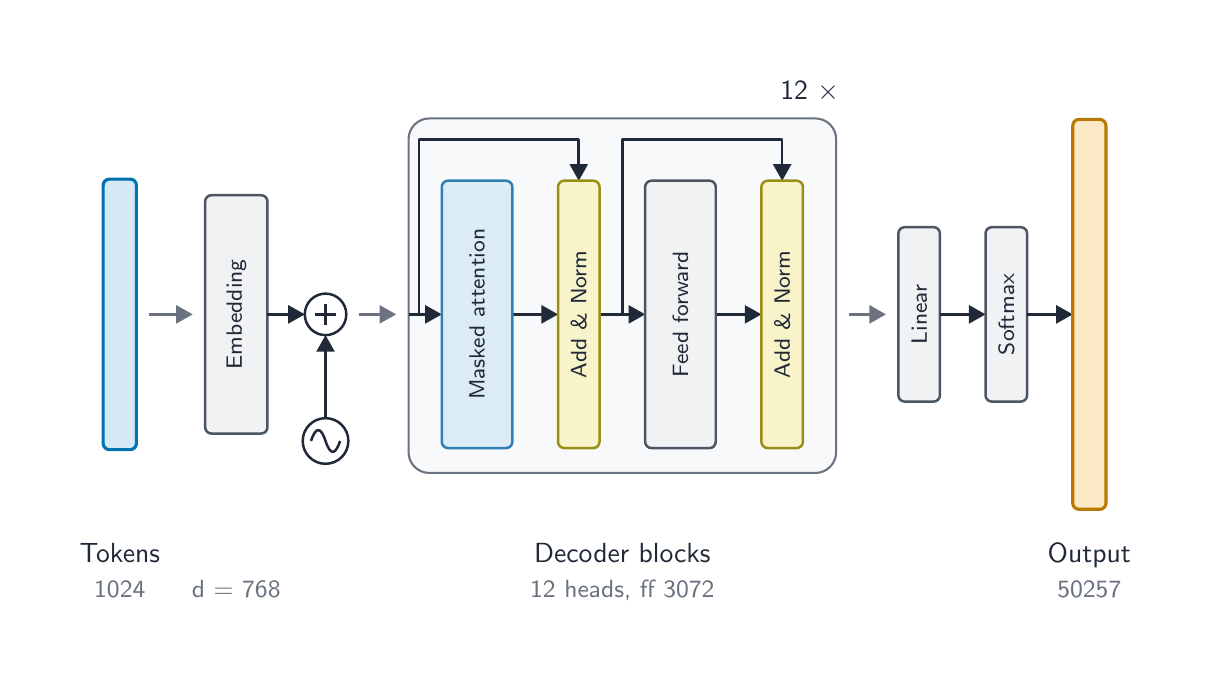
\begin{tikzpicture}[x=0.75pt, y=-0.75pt]
  \tikzset{
    xm arrow d6rgep/.style={draw=xm2, line width=1.05pt},
    xm arrow 14mtdps/.style={fill=xm2, line join=round},
    xm box 1j16zct/.style={fill=xm3, draw=xm4, line width=1.13pt, rounded corners=2.25pt},
    xm box 1ybly7v/.style={fill=xm5, draw=xm6, line width=0.9pt, rounded corners=2.25pt},
    xm text xm7/.style={text=xm7, inner sep=0},
    xm flow 1dxz0x0/.style={draw=xm7, line width=0.95pt},
    xm flow t7rtxn/.style={fill=xm7, line join=round},
    xm op 10yecv/.style={fill=xm1, draw=xm7, line width=0.9pt},
    xm op 19mdedo/.style={draw=xm7, line width=0.98pt, line join=round},
    xm op p0h4fu/.style={draw=xm7, line width=0.9pt, line join=round},
    xm frame 1bupki6/.style={fill=xm8, draw=xm2, line width=0.75pt, rounded corners=7.5pt},
    xm residual 1twkyr3/.style={draw=xm7, line width=0.95pt, line join=round},
    xm residual t7rtxn/.style={fill=xm7, line join=round},
    xm box mghmh4/.style={fill=xm9, draw=xm10, line width=0.9pt, rounded corners=2.25pt},
    xm box 1azwj0l/.style={fill=xm11, draw=xm12, line width=0.9pt, rounded corners=2.25pt},
    xm box bwc7cf/.style={fill=xm13, draw=xm14, line width=1.13pt, rounded corners=2.25pt},
    xm text xm2/.style={text=xm2, inner sep=0},
  }
  \fill[xm1] (0,0) rectangle (554.76,299.3);
  % Diagram
  \path[xm arrow d6rgep] (58.38,138.13) -- (72.51,138.13);
  \path[xm arrow 14mtdps] (79.51,138.13) -- (71.51,142.63) -- (71.51,133.63) -- cycle;
  \path[xm arrow d6rgep] (159.51,138.13) -- (170.51,138.13);
  \path[xm arrow 14mtdps] (177.51,138.13) -- (169.51,142.63) -- (169.51,133.63) -- cycle;
  \path[xm arrow d6rgep] (395.51,138.13) -- (406.51,138.13);
  \path[xm arrow 14mtdps] (413.51,138.13) -- (405.51,142.63) -- (405.51,133.63) -- cycle;
  \path[xm box 1j16zct] (36.38,72.95) rectangle ++(16,130.35);
  \path[xm box 1ybly7v] (85.51,80.73) rectangle ++(30,114.8);
  \node[xm text xm7, font=\sffamily\fontsize{8.25}{9.9}\selectfont, anchor=center, rotate=90] at (100.51,138.13) {Embedding};
  \path[xm flow 1dxz0x0] (115.51,138.13) -- (126.51,138.13);
  \path[xm flow t7rtxn] (133.51,138.13) -- (125.51,142.63) -- (125.51,133.63) -- cycle;
  \path[xm op 10yecv] (143.51,138.13) circle[radius=10];
  \path[xm op 19mdedo] (138.51,138.13) -- (148.51,138.13) (143.51,133.13) -- (143.51,143.13);
  \path[xm flow 1dxz0x0] (143.51,188.13) -- (143.51,155.13);
  \path[xm flow t7rtxn] (143.51,148.13) -- (148.01,156.13) -- (139.01,156.13) -- cycle;
  \path[xm op 10yecv] (143.51,199.13) circle[radius=11];
  \path[xm op p0h4fu] (136.51,199.13) .. controls (138.81,192.13) and (141.21,192.13) .. (143.51,199.13) .. controls (145.81,206.13) and (148.21,206.13) .. (150.51,199.13);
  \path[xm frame 1bupki6] (183.51,43.73) rectangle ++(206,170.8);
  \node[xm text xm7, font=\sffamily\fontsize{9.75}{11.7}\selectfont, anchor=base] at (376.74,34.59) {12 \ensuremath{\times}};
  \path[xm flow 1dxz0x0] (183.51,138.13) -- (192.51,138.13);
  \path[xm flow t7rtxn] (199.51,138.13) -- (191.51,142.63) -- (191.51,133.63) -- cycle;
  \path[xm flow 1dxz0x0] (233.51,138.13) -- (248.51,138.13);
  \path[xm flow t7rtxn] (255.51,138.13) -- (247.51,142.63) -- (247.51,133.63) -- cycle;
  \path[xm flow 1dxz0x0] (275.51,138.13) -- (290.51,138.13);
  \path[xm flow t7rtxn] (297.51,138.13) -- (289.51,142.63) -- (289.51,133.63) -- cycle;
  \path[xm residual 1twkyr3] (188.51,138.13) -- (188.51,53.73) -- (265.51,53.73) -- (265.51,66.73);
  \path[xm residual t7rtxn] (265.51,73.73) -- (261.01,65.73) -- (270.01,65.73) -- cycle;
  \path[xm flow 1dxz0x0] (331.51,138.13) -- (346.51,138.13);
  \path[xm flow t7rtxn] (353.51,138.13) -- (345.51,142.63) -- (345.51,133.63) -- cycle;
  \path[xm residual 1twkyr3] (286.51,138.13) -- (286.51,53.73) -- (363.51,53.73) -- (363.51,66.73);
  \path[xm residual t7rtxn] (363.51,73.73) -- (359.01,65.73) -- (368.01,65.73) -- cycle;
  \path[xm box mghmh4] (199.51,73.73) rectangle ++(34,128.8);
  \node[xm text xm7, font=\sffamily\fontsize{8.25}{9.9}\selectfont, anchor=center, rotate=90] at (216.51,138.13) {Masked attention};
  \path[xm box 1azwj0l] (255.51,73.73) rectangle ++(20,128.8);
  \node[xm text xm7, font=\sffamily\fontsize{8.25}{9.9}\selectfont, anchor=center, rotate=90] at (265.51,138.13) {Add \& Norm};
  \path[xm box 1ybly7v] (297.51,73.73) rectangle ++(34,128.8);
  \node[xm text xm7, font=\sffamily\fontsize{8.25}{9.9}\selectfont, anchor=center, rotate=90] at (314.51,138.13) {Feed forward};
  \path[xm box 1azwj0l] (353.51,73.73) rectangle ++(20,128.8);
  \node[xm text xm7, font=\sffamily\fontsize{8.25}{9.9}\selectfont, anchor=center, rotate=90] at (363.51,138.13) {Add \& Norm};
  \path[xm box 1ybly7v] (419.51,96.13) rectangle ++(20,84);
  \node[xm text xm7, font=\sffamily\fontsize{8.25}{9.9}\selectfont, anchor=center, rotate=90] at (429.51,138.13) {Linear};
  \path[xm flow 1dxz0x0] (439.51,138.13) -- (454.51,138.13);
  \path[xm flow t7rtxn] (461.51,138.13) -- (453.51,142.63) -- (453.51,133.63) -- cycle;
  \path[xm box 1ybly7v] (461.51,96.13) rectangle ++(20,84);
  \node[xm text xm7, font=\sffamily\fontsize{8.25}{9.9}\selectfont, anchor=center, rotate=90] at (471.51,138.13) {Softmax};
  \path[xm flow 1dxz0x0] (481.51,138.13) -- (496.51,138.13);
  \path[xm flow t7rtxn] (503.51,138.13) -- (495.51,142.63) -- (495.51,133.63) -- cycle;
  \path[xm box bwc7cf] (503.51,44.21) rectangle ++(16,187.84);
  \node[xm text xm7, font=\sffamily\fontsize{9.75}{11.7}\selectfont, anchor=base] at (44.38,257.64) {Tokens};
  \node[xm text xm2, font=\sffamily\fontsize{9}{10.8}\selectfont, anchor=base] at (44.38,274.4) {1024};
  \node[xm text xm2, font=\sffamily\fontsize{9}{10.8}\selectfont, anchor=base] at (100.51,274.4) {d = 768};
  \node[xm text xm7, font=\sffamily\fontsize{9.75}{11.7}\selectfont, anchor=base] at (286.51,257.64) {Decoder blocks};
  \node[xm text xm2, font=\sffamily\fontsize{9}{10.8}\selectfont, anchor=base] at (286.51,274.4) {12 heads, ff 3072};
  \node[xm text xm7, font=\sffamily\fontsize{9.75}{11.7}\selectfont, anchor=base] at (511.51,257.64) {Output};
  \node[xm text xm2, font=\sffamily\fontsize{9}{10.8}\selectfont, anchor=base] at (511.51,274.4) {50257};
\end{tikzpicture}
\end{document}
